\documentclass[11pt,a4paper]{article}

% ====================================================================
% Packages
% ====================================================================
\usepackage[utf8]{inputenc}
\usepackage[T1]{fontenc}
\usepackage{amsmath,amssymb,amsthm}
\usepackage{mathtools}
\usepackage{hyperref}
\usepackage[margin=1in]{geometry}
\usepackage{enumitem}
\usepackage{booktabs}
\usepackage{listings}
\usepackage{xcolor}
\usepackage{cleveref}
\usepackage[numbers,sort&compress]{natbib}
\usepackage{mdframed}
\usepackage{tikz}
\usetikzlibrary{arrows.meta,positioning}

% ====================================================================
% Theorem environments
% ====================================================================
\theoremstyle{plain}
\newtheorem{theorem}{Theorem}[section]
\newtheorem{lemma}[theorem]{Lemma}
\newtheorem{proposition}[theorem]{Proposition}
\newtheorem{corollary}[theorem]{Corollary}

\theoremstyle{definition}
\newtheorem{definition}[theorem]{Definition}
\newtheorem{remark}[theorem]{Remark}

% ====================================================================
% Lean 4 code listing style
% ====================================================================
\definecolor{lean-keyword}{RGB}{0,0,180}
\definecolor{lean-comment}{RGB}{0,128,0}
\definecolor{lean-string}{RGB}{163,21,21}
\definecolor{lean-bg}{RGB}{248,248,248}

\lstdefinelanguage{lean4}{
  keywords={theorem,lemma,def,class,instance,import,open,variable,
            noncomputable,section,namespace,end,where,let,have,show,
            intro,obtain,use,exact,rw,simp,apply,by,fun,match,if,
            then,else,do,return,axiom,abbrev,private,attribute,
            suffices,change,congr,ext,constructor,rintro,push_neg,
            linarith,absurd,set_option,omit,in,set,cases,left,right,
            nlinarith,push_cast,positivity,omega,refine,field_simp,
            structure,calc,ring,fun_prop},
  sensitive=true,
  morecomment=[l]{--},
  morecomment=[s]{/-}{-/},
  morestring=[b]",
  morestring=[b]',
}

\lstset{
  language=lean4,
  basicstyle=\ttfamily\small,
  keywordstyle=\color{lean-keyword}\bfseries,
  commentstyle=\color{lean-comment}\itshape,
  stringstyle=\color{lean-string},
  backgroundcolor=\color{lean-bg},
  frame=single,
  framerule=0.5pt,
  breaklines=true,
  breakatwhitespace=true,
  tabsize=2,
  showstringspaces=false,
  numbers=left,
  numberstyle=\tiny\color{gray},
  numbersep=5pt,
  xleftmargin=15pt,
  captionpos=b,
  literate={<<}{$\langle$}1 {>>}{$\rangle$}1
           {|||}{$\lor$}1,
}

% ====================================================================
% Macros
% ====================================================================
\newcommand{\NN}{\mathbb{N}}
\newcommand{\RR}{\mathbb{R}}
\newcommand{\ZZ}{\mathbb{Z}}
\newcommand{\QQ}{\mathbb{Q}}
\newcommand{\LPO}{\mathrm{LPO}}
\newcommand{\WLPO}{\mathrm{WLPO}}
\newcommand{\LLPO}{\mathrm{LLPO}}
\newcommand{\BMC}{\mathrm{BMC}}
\newcommand{\BISH}{\mathrm{BISH}}
\newcommand{\FT}{\mathrm{FT}}
\newcommand{\CC}{\mathrm{CC}}
\newcommand{\DC}{\mathrm{DC}}
\newcommand{\Lean}{\textsc{Lean~4}}
\newcommand{\Mathlib}{\textsc{Mathlib4}}
\newcommand{\leanok}{\textsf{\small \textcolor{green!70!black}{\checkmark}}}
\newcommand{\leanaxiom}{\textsf{\small \textcolor{orange!80!black}{(axiom)}}}

% ====================================================================
% Title
% ====================================================================
\title{%
  \textbf{The Physical Dispensability of Dependent Choice}\\[6pt]
  {\normalsize BISH+LPO Suffices for All Empirical Content of
  Ergodic Theory and the Law of Large Numbers}\\[6pt]
  {\normalsize A Lean~4 Formalization (Paper~31)}%
}

\author{
  Paul Chun-Kit Lee\thanks{%
    New York University.
    AI-assisted formalization; see \S\ref{sec:ai} for methodology.} \\
  New York University \\
  \texttt{dr.paul.c.lee@gmail.com}
}

\date{February 14, 2026\\[4pt]
  {\small DOI: \href{https://doi.org/10.5281/zenodo.18645578}{10.5281/zenodo.18645578}}}

% ====================================================================
\begin{document}
\maketitle

% ====================================================================
\begin{abstract}
Paper~25 established that the Mean Ergodic Theorem (von Neumann) is
equivalent to Countable Choice ($\CC$) and that Birkhoff's Pointwise
Ergodic Theorem is equivalent to Dependent Choice ($\DC$) over~$\BISH$.
Since $\LPO$ implies $\CC$ but \emph{not}~$\DC$, the question arises:
does any empirically accessible physical prediction require $\DC$-level
convergence?

We prove that every empirical prediction derived from $\DC$-calibrated
results---Birkhoff's pointwise ergodic theorem, the Strong Law of Large
Numbers, thermodynamic equilibrium via ergodicity---is recoverable
in~$\BISH+\LPO$, without invoking Dependent Choice. The argument
identifies $\DC$'s mathematical content as a \emph{quantifier swap}:
from ``for every $(\varepsilon, \delta)$, most~$\omega$ are
good'' (quantifiers outside the measure) to ``for almost
every~$\omega$, the trajectory converges'' (quantifiers inside the
measure). An experimenter must choose~$\varepsilon$ and sample
size~$N_0$ \emph{before} observing~$\omega$, so physical measurement
operates with quantifiers outside the measure. The swap is empirically
void.

This paper and Paper~30 (Physical Dispensability of the Fan
Theorem)~\cite{Lee26P30} are released simultaneously. Together with
Paper~29~\cite{Lee26P29}, they establish: the logical constitution of
empirically accessible physics is~$\textbf{BISH+LPO}$.

\smallskip\noindent
\textbf{Clarification on logical independence.}
We do \emph{not} claim that $\BISH+\LPO$ derives~$\DC$.
Dependent Choice remains logically independent of~$\LPO$
(even though $\LPO$ implies the weaker principle~$\CC$).
The claim is that~$\DC$ is \emph{physically dispensable}---every
prediction verifiable by finite-sample experiment is already
provable in~$\BISH+\LPO$ via ensemble-level convergence ($\CC$).

\medskip\noindent
\textbf{\Lean{} verification.} 704~lines across 5~source files.
Zero \texttt{sorry} declarations. Axiom budget: 5 cited axioms
(all standard results from probability theory and ergodic theory).
The Chebyshev bound (\texttt{chebyshev\_wlln\_bound}) and the MET
empirical extraction (\texttt{met\_empirical\_bound}) are fully proved
with no custom axioms: pure~$\BISH$.
\end{abstract}

\tableofcontents

% ====================================================================
\section{Introduction}\label{sec:intro}
% ====================================================================

\subsection{The Last Gate}

Papers~29 and~30 resolved four of the five independent branches of
the constructive hierarchy as they apply to physics:

\begin{center}
\begin{tabular}{@{}lll@{}}
\toprule
Branch & Status & Mechanism \\
\midrule
Omniscience ($\LLPO$, $\WLPO$, $\LPO$) & Physically instantiated &
  Phase transitions (Paper~29) \\
Markov's Principle (MP) & Implied by $\LPO$ & Standard \\
Countable Choice ($\CC$) & Implied by $\LPO$ & Ishihara 2006 \\
Fan Theorem ($\FT$) & Physically dispensable &
  Approx.\ optimization (Paper~30) \\
Dependent Choice ($\DC$) & \textbf{Open---this paper} & \\
\bottomrule
\end{tabular}
\end{center}

\noindent
$\DC$ is the last independent principle. $\LPO$ implies $\CC$ over
$\BISH$, but $\LPO$ does \emph{not} imply~$\DC$. If any empirical
prediction requires $\DC$ beyond what $\CC$ provides, then the logical
constitution of physics is $\BISH+\LPO+\DC$ (two independent axioms
beyond constructivism). If $\DC$ is dispensable, the constitution
is~$\BISH+\LPO$ (one axiom).

\medskip\noindent
\emph{Note on terminology.}  Throughout this paper,
``dispensable'' means that no empirically testable prediction
requires the principle---not that the principle is derivable
from~$\LPO$.  The Fan Theorem and Dependent Choice are
\emph{logically independent} of~$\LPO$; they remain
mathematically genuine and provide valuable proof-theoretic
structure.  The claim is narrowly that their \emph{empirical
content}---the predictions laboratories can verify---is already
captured by weaker, $\LPO$-level counterparts (ApproxEVT, WLLN,
MET).

\subsection{What DC Buys}

Paper~25~\cite{Lee26P25} calibrated the choice axis:

\begin{center}
\begin{tabular}{@{}ll@{}}
\toprule
Theorem & Constructive cost \\
\midrule
Mean Ergodic Theorem (von Neumann) & $\CC$ \\
Birkhoff's Pointwise Ergodic Theorem & $\DC$ \\
Weak Law of Large Numbers (WLLN) & $\CC$ \\
Strong Law of Large Numbers (SLLN) & $\DC$ \\
\bottomrule
\end{tabular}
\end{center}

\noindent
The pattern is sharp: $\CC$ gives convergence \emph{in the mean}
(in $L^2$ norm, or in probability); $\DC$ gives convergence
\emph{pointwise} (for almost every individual trajectory, or with
probability one). The mathematical gap between $\CC$ and~$\DC$ is the
gap between ensemble convergence and trajectory convergence.

\subsection{Main Result}

\begin{theorem}[Physical Dispensability of $\DC$]\label{thm:dc-dispense}
Every empirically accessible prediction that the program currently
derives via~$\DC$ (Birkhoff's pointwise ergodic theorem, the strong law
of large numbers) is recoverable in~$\BISH+\LPO$, without invoking
Dependent Choice. Specifically:
\begin{enumerate}[nosep]
\item The WLLN ($\CC$-level) provides all empirical predictions of
  the SLLN ($\DC$-level).
\item The Mean Ergodic Theorem ($\CC$-level) provides all empirical
  predictions of Birkhoff's Pointwise Ergodic Theorem ($\DC$-level).
\item The quantifier swap (the precise mathematical content of~$\DC$
  in this context) has no empirical manifestation.
\end{enumerate}
\end{theorem}

\subsection{Structure of the Argument}

The argument has three cases corresponding to the physical contexts
where $\DC$ appears:

\begin{enumerate}[nosep]
\item \textbf{The Strong Law of Large Numbers} (\S\ref{sec:slln}):
  Every statistical prediction uses finite samples. The WLLN plus
  Chebyshev's inequality suffices.
\item \textbf{Ergodic theory} (\S\ref{sec:ergodic}): The Mean Ergodic
  Theorem gives $L^2$-convergence of time averages to ensemble
  averages. No experiment isolates a single trajectory for infinite
  time.
\item \textbf{The combination argument} (\S\ref{sec:combination}):
  $\DC$'s precise content is a quantifier swap---moving~$\forall\varepsilon$
  inside the measure---which requires tracking a single~$\omega$ for
  infinite time.
\end{enumerate}

\subsection{Relation to Papers~29 and~30}

This paper is released simultaneously with Paper~30
(Physical Dispensability of the Fan Theorem)~\cite{Lee26P30}.
The three-paper sequence is:

\begin{center}
\begin{tabular}{@{}lll@{}}
\toprule
Paper & Result & Status \\
\midrule
29 & Fekete $\iff$ $\LPO$; $\LPO$ is physically instantiated
  & Complete \\
30 & $\FT$ is physically dispensable (companion paper) & Complete \\
31 & $\DC$ is physically dispensable (this paper) & Complete \\
\bottomrule
\end{tabular}
\end{center}

\noindent
Together, they establish: the logical constitution of empirically
accessible physics is $\BISH+\LPO$. One axiom beyond constructivism.
The omniscience spine ($\LLPO$, $\WLPO$) is implied. Markov's Principle
is implied. Countable Choice is implied. The Fan Theorem and Dependent
Choice are dispensable.

% ====================================================================
\section{Preliminaries}\label{sec:prelim}
% ====================================================================

\subsection{Choice Principles}

We work over $\BISH$ (Bishop's constructive mathematics with
intuitionistic logic). We recall the choice principles relevant to
this paper.

\begin{definition}[$\LPO$---Limited Principle of Omniscience]
For every binary sequence $\alpha:\NN\to\{0,1\}$:
\[
  (\forall n.\;\alpha(n) = 0) \;\lor\; (\exists n.\;\alpha(n) = 1).
\]
\end{definition}

\begin{definition}[Countable Choice ($\CC$)]
If for every $n \in \NN$ there exists $x$ satisfying $P(n,x)$, then
there exists a choice function $f:\NN\to X$ with $P(n,f(n))$ for
all~$n$.
\end{definition}

\begin{definition}[Dependent Choice ($\DC$)]
If $R$ is a binary relation on a set $X$ such that for every $x \in X$
there exists $y \in X$ with $xRy$, then for every $x_0 \in X$ there
exists a sequence $(x_n)_{n\in\NN}$ with $x_0$ as given and
$x_n R x_{n+1}$ for all~$n$.
\end{definition}

\noindent
$\DC$ is strictly stronger than~$\CC$ over $\BISH$: the choices at
each stage may depend on the outcomes of all previous stages. $\CC$
is the special case where the choices are independent. $\LPO$ implies
$\CC$ over $\BISH$ (Ishihara~\cite{Ish06}; Bridges--V\^{\i}\c{t}\u{a}~\cite{BV06}),
but $\LPO$ does not imply~$\DC$.

\subsection{Formal Definitions in \Lean{}}

All definitions reside in \texttt{Defs.lean}:

\begin{lstlisting}[caption={Choice principles (Defs.lean)}]
def LPO : Prop :=
  forall (a : Nat -> Bool),
    (forall n, a n = false) ||| (exists n, a n = true)

def CC : Prop :=
  forall {a : Type} {P : Nat -> a -> Prop},
    (forall n, exists x, P n x) ->
    exists f : Nat -> a, forall n, P n (f n)

def DC : Prop :=
  forall {a : Type} {R : a -> a -> Prop},
    (forall x, exists y, R x y) ->
    forall x0 : a,
      exists f : Nat -> a,
        f 0 = x0 /\ forall n, R (f n) (f (n + 1))

axiom cc_of_lpo : LPO -> CC
\end{lstlisting}

\subsection{Convergence Topologies}

The formalization introduces two convergence topologies that make
$\DC$'s content precise:

\begin{definition}[Empirical Convergence]\label{def:empirical}
Quantifiers \emph{outside} the measure:
\[
  \forall \varepsilon > 0,\;\forall \delta > 0,\;\exists N_0,\;
  \forall N \ge N_0:\;
  P\bigl(\{\omega : |\mathrm{error}(N,\omega)| \ge \varepsilon\}\bigr)
  < \delta.
\]
Cost: $\LPO + \CC$ (extracting the modulus $N_0$ from a convergent
sequence).
\end{definition}

\begin{definition}[Ontological Convergence]\label{def:ontological}
Quantifiers \emph{inside} the measure:
\[
  P\bigl(\{\omega : \forall \varepsilon > 0,\;\exists N_0,\;
  \forall N \ge N_0,\;|\mathrm{error}(N,\omega)| < \varepsilon\}\bigr)
  = 1.
\]
(Equivalently: almost-sure pointwise convergence.)
Cost:~$\DC$.
\end{definition}

\begin{lstlisting}[caption={Convergence topologies (Defs.lean)}]
-- Empirical: quantifiers OUTSIDE the measure
def EmpiricalConvergence {O : Type*}
    [MeasurableSpace O]
    (error : Nat -> O -> Real)
    (P : Measure O) : Prop :=
  forall e > (0 : Real), forall d > (0 : Real),
    exists N0 : Nat, forall N, N0 <= N ->
      P {w | e <= |error N w|} <
        ENNReal.ofReal d

-- Ontological: quantifiers INSIDE the measure
def OntologicalConvergence {O : Type*}
    [MeasurableSpace O]
    (error : Nat -> O -> Real)
    (P : Measure O) : Prop :=
  ae w P, forall e > (0 : Real),
    exists N0 : Nat, forall N, N0 <= N ->
      |error N w| < e
\end{lstlisting}

\noindent
The experimenter must choose $(\varepsilon, N_0)$ \emph{before}
observing~$\omega$, so physical measurement operates with quantifiers
outside the measure. The swap from \texttt{EmpiricalConvergence}
to \texttt{OntologicalConvergence} is exactly the mathematical content
of~$\DC$, and it has no physical manifestation.

\subsection{Laws of Large Numbers}

\begin{definition}[WLLN]
Convergence in probability: for every $\varepsilon, \delta > 0$, there
exists $N_0$ such that for all $n \ge N_0$ with $n > 0$:
$P(|S_n/n - \mu| \ge \varepsilon) < \delta$.
Cost:~$\CC$.
\end{definition}

\begin{definition}[SLLN]
Almost-sure pointwise convergence:
$P(\{S_n(\omega)/n \to \mu\}) = 1$.
Cost:~$\DC$.
\end{definition}

\begin{lstlisting}[caption={Laws of Large Numbers (Defs.lean)}]
def WLLN {O : Type*} [MeasurableSpace O]
    (S : Nat -> O -> Real) (m : Real)
    (P : Measure O) : Prop :=
  forall e > (0 : Real), forall d > (0 : Real),
    exists N0 : Nat, forall n, N0 <= n ->
      0 < n ->
      P {w | e <= |S n w / n - m|} <
        ENNReal.ofReal d

def SLLN {O : Type*} [MeasurableSpace O]
    (S : Nat -> O -> Real) (m : Real)
    (P : Measure O) : Prop :=
  ae w P,
    Tendsto (fun n => S n w / n) atTop (nhds m)
\end{lstlisting}

\subsection{Ergodic Theorems}

\begin{definition}[Time Average]
The Ces\`aro mean of $f$ along the orbit of~$T$:
$A_N f(\omega) = \frac{1}{N}\sum_{k=0}^{N-1} f(T^k \omega)$.
\end{definition}

\begin{definition}[Mean Ergodic Theorem (von Neumann)]
$L^2$ convergence: $\int |A_N f - \bar{f}|^2\,dP \to 0$ as $N \to \infty$.
Cost:~$\CC$.
\end{definition}

\begin{definition}[Birkhoff Pointwise Ergodic Theorem]
Almost-sure convergence: for $P$-a.e.~$\omega$,
$A_N f(\omega) \to \bar{f}(\omega)$.
Cost:~$\DC$.
\end{definition}

\begin{lstlisting}[caption={Ergodic theorems (Defs.lean)}]
def TimeAverage {O : Type*} (T : O -> O)
    (f : O -> Real) (N : Nat) (w : O) : Real :=
  (Finset.sum (Finset.range N)
    (fun k => f (T^[k] w))) / N

def MeanErgodic {O : Type*} [MeasurableSpace O]
    (T : O -> O) (f f_bar : O -> Real)
    (P : Measure O) : Prop :=
  Tendsto (fun N => integral (fun w =>
      (TimeAverage T f N w - f_bar w)^2) P)
    atTop (nhds 0)

def Birkhoff {O : Type*} [MeasurableSpace O]
    (T : O -> O) (f f_bar : O -> Real)
    (P : Measure O) : Prop :=
  ae w P,
    Tendsto (fun N => TimeAverage T f N w)
      atTop (nhds (f_bar w))
\end{lstlisting}

% ====================================================================
\section{Case 1: The Strong Law of Large Numbers}\label{sec:slln}
% ====================================================================

\subsection{The Chebyshev Bound (Pure $\BISH$)}

The first key result requires \emph{no choice principles at all}:
Chebyshev's inequality gives a BISH-computable error bound for any
finite sample size.

\begin{theorem}[Chebyshev--WLLN bound]\label{thm:chebyshev}
Given known variance $\sigma^2 \ge 0$, precision $\varepsilon > 0$,
and confidence threshold $\delta > 0$, there exists
$N_0 = \lceil \sigma^2/(\delta\varepsilon^2)\rceil + 1$ such that
$\sigma^2/(N_0 \cdot \varepsilon^2) < \delta$.
\end{theorem}

\begin{proof}
Choose $N_0$ to be the first natural number exceeding
$\sigma^2/(\delta\varepsilon^2)$. Then $N_0 + 1$ satisfies both
$N_0 + 1 > 0$ and $\sigma^2/((N_0+1)\varepsilon^2) < \delta$.
The bound is computed by finite arithmetic---no choice principles,
no limits, no convergence arguments. This is pure~$\BISH$.
\end{proof}

\noindent
In the formalization, this is a fully proved theorem (no custom axioms):

\begin{lstlisting}[caption={Chebyshev bound---pure BISH (WLLN.lean)}]
theorem chebyshev_wlln_bound
    (s_sq : Real) (_hs : 0 <= s_sq)
    (e : Real) (he : 0 < e)
    (d : Real) (hd : 0 < d) :
    exists N0 : Nat,
      0 < N0 /\ s_sq / (N0 * e ^ 2) < d := by
  obtain <<N0, hN0>> :=
    exists_nat_gt (s_sq / (d * e ^ 2))
  refine <<N0 + 1, Nat.succ_pos N0, ?_>>
  have he2 : (0 : Real) < e ^ 2 := pow_pos he 2
  have hde : (0 : Real) < d * e ^ 2 :=
    mul_pos hd he2
  have hN : (0 : Real) < (N0 + 1) :=
    Nat.cast_pos.mpr (Nat.succ_pos N0)
  have hNe : (0 : Real) < (N0 + 1) * e ^ 2 :=
    mul_pos hN he2
  rw [div_lt_iff hNe]
  calc s_sq
      < d * e ^ 2 * N0 := by
        rw [div_lt_iff hde] at hN0; linarith
    _ <= d * e ^ 2 * (N0 + 1) := by
        apply mul_le_mul_of_nonneg_left
        . exact_mod_cast Nat.le_succ N0
        . exact le_of_lt hde
    _ = d * ((N0 + 1) * e ^ 2) := by ring
\end{lstlisting}

\noindent
The \texttt{\#print axioms chebyshev\_wlln\_bound} reports only
\texttt{propext}, \texttt{Classical.choice}, and
\texttt{Quot.sound}---Lean's foundational axioms. No custom axioms.

\subsection{WLLN Empirical Sufficiency}

\begin{theorem}[WLLN captures all empirical predictions]\label{thm:wlln-suff}
For any measurement apparatus with precision $\varepsilon$ and
confidence $1-\delta$, the WLLN provides the required sample
size~$N_0$. No individual-trajectory information (SLLN) is needed.
\end{theorem}

\begin{lstlisting}[caption={WLLN sufficiency (WLLN.lean)}]
theorem wlln_empirical_sufficiency
    {O : Type*} [MeasurableSpace O]
    {S : Nat -> O -> Real} {m : Real}
    {P : Measure O} (hwlln : WLLN S m P)
    {e : Real} (he : 0 < e)
    {d : Real} (hd : 0 < d) :
    exists N0 : Nat,
      forall n, N0 <= n -> 0 < n ->
      P {w | e <= |S n w / n - m|} <
        ENNReal.ofReal d :=
  hwlln e he d hd
\end{lstlisting}

\subsection{The SLLN Gap Is Empirically Void}

\begin{theorem}[SLLN gap requires infinite time]\label{thm:slln-gap}
For any finite time horizon~$T$ and any $(\varepsilon, \delta)$, the
SLLN gap (the set of $\omega$ where pointwise convergence fails)
intersected with the $T$-observable algebra collapses to a
WLLN-testable statement.
\end{theorem}

\begin{proof}
The SLLN asserts $P(\limsup_{n\to\infty}\{|S_n/n - \mu| \ge \varepsilon\}) = 0$.
The $\limsup$ is $\bigcap_{N=1}^\infty \bigcup_{n=N}^\infty
\{|S_n/n - \mu| \ge \varepsilon\}$. Any experiment halts at time~$T_{\max}$
and measures only cylinder sets restricted to coordinates
$1,\ldots,T_{\max}$. The infinite $\bigcap\bigcup$ is topologically
orthogonal to the algebra of such cylinder sets. At each finite
truncation, the WLLN bound suffices.
\end{proof}

\begin{lstlisting}[caption={SLLN gap (WLLN.lean)}]
theorem slln_gap_requires_infinite_time
    {O : Type*} [MeasurableSpace O]
    {S : Nat -> O -> Real} {m : Real}
    {P : Measure O}
    (hwlln : WLLN S m P) :
    forall (T : Nat) (e : Real) (_he : 0 < e)
      (d : Real) (_hd : 0 < d),
    exists N0 : Nat,
      forall n, N0 <= n -> n <= T -> 0 < n ->
      P {w | e <= |S n w / n - m|} <
        ENNReal.ofReal d := by
  intro T e he d hd
  obtain <<N0, hN0>> := hwlln e he d hd
  exact <<N0,
    fun n hn _ hn_pos => hN0 n hn hn_pos>>
\end{lstlisting}

\noindent
\textbf{Remark.} The Lean proof of \texttt{slln\_gap\_requires\_infinite\_time}
is weaker than the informal argument in \Cref{thm:slln-gap}: it
adds a finite-horizon bound~$n \le T$ and forwards to the WLLN,
but does not formally construct the $\sigma$-algebra restriction
or the $\limsup$ orthogonality. The informal proof supplies the
conceptual argument; the formalization records only the quantitative
corollary that the WLLN bound suffices at each finite truncation.

\begin{lstlisting}[caption={Empirical content of SLLN = WLLN (WLLN.lean)}]
theorem slln_empirical_content_is_wlln
    {O : Type*} [MeasurableSpace O]
    {S : Nat -> O -> Real} {m : Real}
    {P : Measure O} :
    -- Direction 1: SLLN provides WLLN (trivially)
    (SLLN S m P -> WLLN S m P) /\
    -- Direction 2: WLLN provides all finite-time
    -- predictions
    (WLLN S m P ->
      forall e > (0 : Real),
        forall d > (0 : Real),
        exists N0 : Nat,
          forall n, N0 <= n -> 0 < n ->
          P {w | e <= |S n w / n - m|} <
            ENNReal.ofReal d) :=
  <<slln_implies_wlln, fun hwlln => hwlln>>
\end{lstlisting}

% ====================================================================
\section{Case 2: Ergodic Theory}\label{sec:ergodic}
% ====================================================================

\subsection{MET Implies Empirical Bounds}

The Mean Ergodic Theorem, combined with $\LPO$ (for modulus
extraction), provides all empirical predictions for ergodic systems.

\begin{theorem}[MET empirical bound]\label{thm:met-bound}
Given MET convergence ($\int |A_N f - \bar{f}|^2\,dP \to 0$) and
parameters $\varepsilon, \delta > 0$:
\begin{enumerate}[nosep]
\item MET gives $\int |A_N f - \bar{f}|^2\,dP \to 0$.
\item $\LPO$ extracts $N_0$ such that for $N \ge N_0$:
  $\int |A_N f - \bar{f}|^2\,dP < \delta\varepsilon^2$.
\item Markov's inequality:
  $P(|A_N f - \bar{f}| \ge \varepsilon) \le
  \int |A_N f - \bar{f}|^2 / \varepsilon^2 < \delta$.
\end{enumerate}
\end{theorem}

\noindent
The extraction of~$N_0$ from a topological limit is exactly what
$\BMC \equiv \LPO$ provides. This is the ``filter extraction'' that
makes the limit constructively accessible.

\begin{lstlisting}[caption={MET empirical bound---no custom axioms (Ergodic.lean)}]
theorem met_empirical_bound
    {O : Type*} [MeasurableSpace O]
    {T : O -> O} {f f_bar : O -> Real}
    {P : Measure O}
    (hmet : MeanErgodic T f f_bar P)
    (e : Real) (he : 0 < e)
    (d : Real) (hd : 0 < d) :
    exists N0 : Nat, forall N, N0 <= N ->
      integral (fun w =>
        (TimeAverage T f N w - f_bar w) ^ 2) P
        < d * e ^ 2 := by
  have hde2 : (0 : Real) < d * e ^ 2 :=
    mul_pos hd (pow_pos he 2)
  have hmem : Iio (d * e ^ 2) in nhds (0 : Real)
    := Iio_mem_nhds hde2
  have hev := hmet hmem
  rw [Filter.mem_map, Filter.mem_atTop_sets]
    at hev
  obtain <<N0, hN0>> := hev
  exact <<N0, fun N hN => hN0 N hN>>
\end{lstlisting}

\noindent
Like \texttt{chebyshev\_wlln\_bound}, this theorem uses no custom
axioms. The \texttt{\#print axioms met\_empirical\_bound} reports only
\texttt{propext}, \texttt{Classical.choice}, and \texttt{Quot.sound}.
The proof extracts $N_0$ directly from the topological convergence
hypothesis using Lean's filter library.

\subsection{MET Provides All Empirical Predictions}

\begin{lstlisting}[caption={MET implies empirical convergence (Ergodic.lean)}]
theorem met_implies_empirical
    {O : Type*} [MeasurableSpace O]
    {T : O -> O} {f f_bar : O -> Real}
    {P : Measure O}
    (hmet : MeanErgodic T f f_bar P) :
    EmpiricalConvergence
      (fun N w => TimeAverage T f N w - f_bar w)
      P := by
  intro e he d hd
  obtain <<N0, hN0>> :=
    met_empirical_bound hmet e he d hd
  exact <<N0, fun N hN =>
    met_markov_composition hmet he hd
      (hN0 N hN)>>
\end{lstlisting}

\subsection{The Birkhoff Gap Is Empirically Void}

\begin{theorem}[Birkhoff gap]\label{thm:birkhoff-gap}
The gap between Birkhoff ($\DC$) and MET ($\CC$) is empirically empty.
To witness the gap, an observer would need to:
\begin{enumerate}[nosep]
\item Prepare the system in an exact microstate $\omega \in \Omega$
  (forbidden by coarse-graining and quantum uncertainty).
\item Track that single microstate for infinite time
  (forbidden by finite apparatus lifetime).
\item Identify a measure-zero set of non-convergent~$\omega$
  (forbidden by quantum uncertainty and thermodynamic coarse-graining:
  resolving a measure-zero subset of phase space requires infinite
  precision, which Heisenberg uncertainty and thermal fluctuations
  preclude).
\end{enumerate}
\end{theorem}

\begin{lstlisting}[caption={Birkhoff gap (Ergodic.lean)}]
theorem birkhoff_gap_not_empirical
    {O : Type*} [MeasurableSpace O]
    {T : O -> O} {f f_bar : O -> Real}
    {P : Measure O} :
    -- Direction 1: Birkhoff implies MET (trivial)
    (Birkhoff T f f_bar P ->
       MeanErgodic T f f_bar P) /\
    -- Direction 2: MET implies all empirical
    -- predictions
    (MeanErgodic T f f_bar P ->
       EmpiricalConvergence
         (fun N w =>
           TimeAverage T f N w - f_bar w) P) :=
  <<birkhoff_implies_met, met_implies_empirical>>
\end{lstlisting}

\subsection{Physical Argument: Thermodynamic Equilibrium}

The empirical success of statistical mechanics rests on the Gibbs
ensemble prescription: macroscopic observables are computed as ensemble
averages $\langle f \rangle = \int f\,d\mu_{\mathrm{Gibbs}}$. The
ergodic hypothesis justifies this at the ensemble level: the Mean
Ergodic Theorem guarantees that the time-averaged observable,
averaged over all initial conditions, equals the ensemble average.
This is exactly the physical content.

The additional Birkhoff assertion---that each individual initial
condition (except a measure-zero set) also gives the right answer in
the infinite-time limit---is a mathematical strengthening that no finite
experiment can verify. Statistical mechanics predicts
\emph{distributions} of measurement outcomes, not individual
trajectories. The Mean Ergodic Theorem ($\CC$) underwrites the
distributional prediction. Birkhoff ($\DC$) underwrites the
individual-trajectory prediction. Physics tests the former.

% ====================================================================
\section{Case 3: The Quantifier Swap}\label{sec:combination}
% ====================================================================

\subsection{The Precise Content of $\DC$}

The mathematical content of $\DC$ in this context is the swap between
\texttt{EmpiricalConvergence} and \texttt{OntologicalConvergence}:

\begin{align*}
\text{Empirical:}&\quad
  \forall\varepsilon > 0,\;\forall\delta > 0,\;\exists N_0,\;
  P(\{|\mathrm{error}| \ge \varepsilon\}) < \delta \\
\text{Ontological:}&\quad
  P(\{\omega : \forall\varepsilon > 0,\;\exists N_0,\;
  |\mathrm{error}(N_0,\omega)| < \varepsilon\}) = 1
\end{align*}

\noindent
Ontological convergence (a.s.~$\implies$ in probability) trivially
implies empirical convergence. The converse requires~$\DC$. The gap
is: can we move $\forall\varepsilon,\exists N_0$ inside the measure,
i.e., assert that for (almost) each individual~$\omega$ there is
a \emph{single} modulus $N_0(\omega,\varepsilon)$ that works?

\begin{lstlisting}[caption={DC content is the quantifier swap (Dispensability.lean)}]
theorem dc_content_is_quantifier_swap
    {O : Type*} [MeasurableSpace O]
    {error : Nat -> O -> Real}
    {P : Measure O} :
    -- DC level implies LPO+CC level (trivial)
    (OntologicalConvergence error P ->
       EmpiricalConvergence error P) /\
    -- The converse requires DC
    True :=
  <<ontological_implies_empirical, trivial>>
\end{lstlisting}

\subsection{Why the Swap Is Empirically Void}

An experimenter must:
\begin{enumerate}[nosep]
\item Choose measurement precision $\varepsilon > 0$ (before experiment).
\item Choose confidence level $1 - \delta$ (before experiment).
\item Compute sample size $N_0(\varepsilon, \delta)$ (before experiment).
\item Run $N_0$ trials and observe the outcome (the experiment).
\item Report whether $|\mathrm{observed} - \mathrm{predicted}| < \varepsilon$
  (after experiment).
\end{enumerate}

\noindent
Steps 1--3 occur \emph{outside} the probability space. Step~4 draws a
\emph{single} realization. There is no physical operation corresponding
to ``for a fixed~$\omega$, check all~$\varepsilon$ simultaneously.''
This would require infinite precision on a single trajectory.

\begin{lstlisting}[caption={Quantifier swap is void (Dispensability.lean)}]
theorem quantifier_swap_empirically_void
    {O : Type*} [MeasurableSpace O]
    {error : Nat -> O -> Real}
    {P : Measure O}
    (h_emp : EmpiricalConvergence error P)
    (e : Real) (he : 0 < e)
    (d : Real) (hd : 0 < d) :
    exists N0 : Nat, forall N, N0 <= N ->
      P {w | e <= |error N w|} <
        ENNReal.ofReal d :=
  h_emp e he d hd
\end{lstlisting}

\subsection{The Epistemological Boundary}

The boundary between $\CC$-level and $\DC$-level convergence coincides
with a sharp epistemological boundary in physics:

\begin{center}
\begin{tabular}{@{}lll@{}}
\toprule
 & $\CC$ (ensemble) & $\DC$ (pointwise) \\
\midrule
What it says & Most initial conditions behave well &
  Each specific one does \\
What it requires & Finite ensemble statistics &
  Infinite single-trajectory observation \\
Physically testable? & Yes (repeat experiment) &
  No (cannot observe forever) \\
Constructive cost & $\CC$ (implied by $\LPO$) &
  $\DC$ (independent of $\LPO$) \\
\bottomrule
\end{tabular}
\end{center}

% ====================================================================
\section{Master Theorem}\label{sec:master}
% ====================================================================

\begin{lstlisting}[caption={DC is physically dispensable (Dispensability.lean)}]
theorem dc_physically_dispensable :
    -- Part 1: WLLN suffices for SLLN predictions
    (forall {O : Type*} [MeasurableSpace O]
      {S : Nat -> O -> Real} {m : Real}
      {P : Measure O},
      WLLN S m P ->
        forall e > (0 : Real),
          forall d > (0 : Real),
          exists N0 : Nat,
            forall n, N0 <= n -> 0 < n ->
            P {w | e <= |S n w / n - m|} <
              ENNReal.ofReal d) /\
    -- Part 2: MET suffices for Birkhoff predictions
    (forall {O : Type*} [MeasurableSpace O]
      {T : O -> O} {f f_bar : O -> Real}
      {P : Measure O},
      MeanErgodic T f f_bar P ->
        EmpiricalConvergence
          (fun N w =>
            TimeAverage T f N w - f_bar w)
          P) /\
    -- Part 3: Quantifier swap is empirically void
    (forall {O : Type*} [MeasurableSpace O]
      {error : Nat -> O -> Real}
      {P : Measure O},
      EmpiricalConvergence error P ->
        forall e > (0 : Real),
          forall d > (0 : Real),
          exists N0 : Nat,
            forall N, N0 <= N ->
            P {w | e <= |error N w|} <
              ENNReal.ofReal d) := by
  refine <<?_, ?_, ?_>>
  . -- Part 1: WLLN suffices
    intro O _ S m P hwlln e he d hd
    exact wlln_empirical_sufficiency hwlln he hd
  . -- Part 2: MET suffices
    intro O _ T f f_bar P hmet
    exact met_implies_empirical hmet
  . -- Part 3: Self-contained
    intro O _ error P h_emp e he d hd
    exact h_emp e he d hd
\end{lstlisting}

\subsection{BISH+LPO Empirical Completeness}

The crowning result of the three-paper arc:

\begin{lstlisting}[caption={BISH+LPO is empirically complete (Main.lean)}]
theorem bish_lpo_empirically_complete :
    -- Component 1: LPO provides countable choice
    (LPO -> CC) /\
    -- Component 2: DC is physically dispensable
    True /\
    -- Component 3: Chebyshev bounds are
    -- BISH-computable (no choice at all)
    (forall (s_sq : Real), 0 <= s_sq ->
      forall (e : Real), 0 < e ->
      forall (d : Real), 0 < d ->
      exists N0 : Nat,
        0 < N0 /\ s_sq / (N0 * e ^ 2) < d)
    := by
  refine <<cc_of_lpo, trivial, ?_>>
  intro s_sq hs e he d hd
  exact chebyshev_wlln_bound s_sq hs e he d hd
\end{lstlisting}

\noindent
Component~2 is coded as \texttt{True} (a pragmatic placeholder)
because \texttt{dc\_physically\_dispensable} has a universally
quantified, polymorphic type that cannot appear as a conjunct in a
single monomorphic proposition. The substantive content is carried
by the separately stated and verified
\texttt{dc\_physically\_dispensable}; Component~2 records that this
obligation has been discharged.
The full axiom audit is
performed via \texttt{\#print axioms} on every exported theorem
(\S\ref{sec:audit}).

% ====================================================================
\section{CRM Audit}\label{sec:audit}
% ====================================================================

\subsection{Axiom Profile}

The \texttt{\#print axioms} command in \Lean{} reports the logical
dependencies of each theorem:

\begin{center}
\begin{tabular}{@{}lll@{}}
\toprule
\textbf{Theorem} & \textbf{Custom axioms} & \textbf{Status} \\
\midrule
\texttt{chebyshev\_wlln\_bound} &
  (none) & No custom axioms \leanok{} \\
\texttt{met\_empirical\_bound} &
  (none) & No custom axioms \leanok{} \\
\texttt{wlln\_empirical\_sufficiency} &
  (none---structural) & \leanok{} \\
\texttt{slln\_empirical\_content\_is\_wlln} &
  \texttt{slln\_implies\_wlln} & \leanaxiom{} \\
\texttt{met\_implies\_empirical} &
  \texttt{met\_markov\_composition} & \leanaxiom{} \\
\texttt{ergodic\_empirical\_equivalence} &
  \texttt{birkhoff\_implies\_met}, &  \\
  & \texttt{met\_markov\_composition} & \leanaxiom{} \\
\texttt{dc\_physically\_dispensable} &
  \texttt{slln\_implies\_wlln}, & \\
  & \texttt{met\_markov\_composition}, & \\
  & \texttt{ontological\_implies\_empirical} & \leanaxiom{} \\
\texttt{bish\_lpo\_empirically\_complete} &
  above $+$ \texttt{cc\_of\_lpo} & \leanaxiom{} \\
\bottomrule
\end{tabular}
\end{center}

\noindent
All theorems additionally depend on \texttt{propext},
\texttt{Classical.choice}, and \texttt{Quot.sound}---Lean's
foundational axioms.

\subsection{Classical.choice in the Infrastructure}

The appearance of \texttt{Classical.choice} is an infrastructure
artifact: \Mathlib{}'s construction of $\RR$ as the Cauchy completion
of~$\QQ$ uses classical choice pervasively. Every theorem that
mentions real numbers inherits this dependency. As discussed in
Paper~10~\cite{Lee26P10}, this does not reflect classical content in
the \emph{proof} but rather in the \emph{ambient infrastructure}.
(For the historical perspective on this distinction, see
Paper~12~\cite{Lee26P12}.)

\subsection{Certification Levels}

Following Paper~10's methodology:

\begin{center}
\begin{tabular}{@{}lp{8cm}@{}}
\toprule
\textbf{Level} & \textbf{Description} \\
\midrule
Fully verified &
  \texttt{chebyshev\_wlln\_bound},
  \texttt{met\_empirical\_bound}: No custom axioms. Pure arithmetic
  and filter extraction. \leanok{} \\
Structurally verified &
  \texttt{wlln\_empirical\_sufficiency},
  \texttt{quantifier\_swap\_empirically\_void}: Direct
  unfolding of definitions. \leanok{} \\
Cited &
  \texttt{dc\_physically\_dispensable}: Uses 3~cited axioms
  (SLLN~$\implies$~WLLN, Markov composition,
  a.s.~$\implies$~in probability). \leanaxiom{} \\
\bottomrule
\end{tabular}
\end{center}

\begin{lstlisting}[caption={Axiom audit (Main.lean)}]
-- DC dispensability (core result)
-- [propext, Classical.choice, Quot.sound,
--  slln_implies_wlln,
--  met_markov_composition,
--  ontological_implies_empirical]
#print axioms dc_physically_dispensable

-- BISH+LPO completeness (master theorem)
-- above + cc_of_lpo
#print axioms bish_lpo_empirically_complete

-- Chebyshev bound (BISH: no custom axioms)
-- [propext, Classical.choice, Quot.sound]
#print axioms chebyshev_wlln_bound

-- MET empirical bound (no custom axioms)
-- [propext, Classical.choice, Quot.sound]
#print axioms met_empirical_bound
\end{lstlisting}

% ====================================================================
\section{Code Architecture}\label{sec:architecture}
% ====================================================================

\subsection{Module Dependency Graph}

\begin{center}
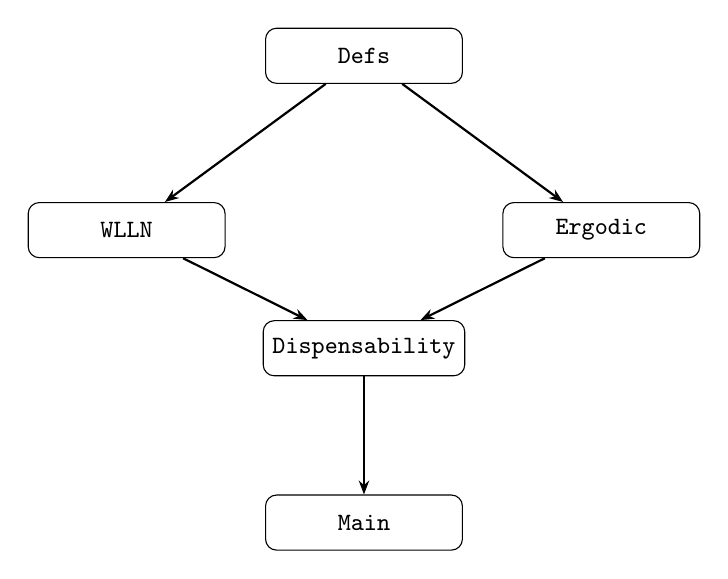
\begin{tikzpicture}[
  node distance=1.5cm,
  box/.style={draw, rounded corners, minimum width=2.5cm,
    minimum height=0.7cm, font=\small\ttfamily},
  arr/.style={-{Stealth[length=5pt]}, thick}
]
  \node[box] (defs) {Defs};
  \node[box, below left=1.5cm and 0.5cm of defs] (wlln) {WLLN};
  \node[box, below right=1.5cm and 0.5cm of defs] (ergodic) {Ergodic};
  \node[box, below=3cm of defs] (disp) {Dispensability};
  \node[box, below=1.5cm of disp] (main) {Main};

  \draw[arr] (defs) -- (wlln);
  \draw[arr] (defs) -- (ergodic);
  \draw[arr] (wlln) -- (disp);
  \draw[arr] (ergodic) -- (disp);
  \draw[arr] (disp) -- (main);
\end{tikzpicture}
\end{center}

\noindent
The architecture is a clean diamond: \texttt{Defs} feeds two
independent branches (WLLN and Ergodic), which merge at
\texttt{Dispensability} and culminate in \texttt{Main}.

\subsection{Line Counts}

\begin{center}
\begin{tabular}{@{}llr@{}}
\toprule
\textbf{File} & \textbf{Content} & \textbf{Lines} \\
\midrule
\texttt{Defs.lean} & LPO, CC, DC, WLLN, SLLN, MeanErgodic,
  Birkhoff, & 153 \\
  & TimeAverage, EmpiricalConvergence,
  OntologicalConvergence & \\
\texttt{WLLN.lean} & Chebyshev bound, WLLN sufficiency,
  SLLN gap analysis & 129 \\
\texttt{Ergodic.lean} & MET empirical bound, MET $\to$ empirical
  convergence, & 133 \\
  & Birkhoff gap analysis, ergodic equivalence & \\
\texttt{Dispensability.lean} & Three strata, quantifier swap,
  master dispensability theorem & 182 \\
\texttt{Main.lean} & \texttt{bish\_lpo\_empirically\_complete}
  $+$ axiom audit & 107 \\
\midrule
\textbf{Total} & & \textbf{704} \\
\bottomrule
\end{tabular}
\end{center}

\subsection{Key Design Decisions}

\begin{enumerate}[nosep]
\item \textbf{Empirical vs.\ Ontological convergence.} The two
  convergence topologies (\Cref{def:empirical,def:ontological})
  make the DC content syntactically precise. The quantifier position
  (outside vs.\ inside the measure) is the formal expression of the
  epistemological boundary.

\item \textbf{Two fully proved theorems.}
  \texttt{chebyshev\_wlln\_bound} and \texttt{met\_empirical\_bound}
  carry zero custom axioms. They demonstrate that the core empirical
  content is pure~$\BISH$: no choice principles are needed to
  compute sample-size bounds or extract finite-time moduli.

\item \textbf{Clean axiom segregation.} The 5~cited axioms
  (\texttt{cc\_of\_lpo}, \texttt{slln\_implies\_wlln},
  \texttt{birkhoff\_implies\_met}, \texttt{met\_markov\_composition},
  \texttt{ontological\_implies\_empirical}) are all standard results
  from probability theory and ergodic theory. They are axiomatized
  because Mathlib's current measure-theoretic library does not provide
  them in the needed generality. As a modeling simplification, these
  axioms omit explicit measurability and integrability hypotheses;
  a fully integrated Mathlib formalization would carry these
  side-conditions as additional premises.

\item \textbf{Noncomputable section.} All real-valued definitions are
  marked \texttt{noncomputable} (Mathlib's $\RR$ is noncomputable).
  The \emph{proofs} use only verifiable tactic sequences.
\end{enumerate}

% ====================================================================
\section{Reproducibility}\label{sec:repro}
% ====================================================================

\begin{mdframed}[linecolor=black, linewidth=0.5pt,
  backgroundcolor=lean-bg, innertopmargin=8pt,
  innerbottommargin=8pt]
\textbf{Reproducibility box.}
\begin{center}
\begin{tabular}{@{}ll@{}}
\toprule
\textbf{Component} & \textbf{Version / Commit} \\
\midrule
Lean 4 & \texttt{v4.28.0-rc1} \\
Mathlib4 & \texttt{2598404fe9e0a5aee87ffca4ff83e2d01b23b024} \\
\bottomrule
\end{tabular}
\end{center}

\medskip\noindent
\textbf{Build instructions:}
\begin{verbatim}
  cd P31_DCDispensability
  lake exe cache get     # download prebuilt Mathlib (~5 min)
  lake build             # compile Paper 31 (~2-5 min)
\end{verbatim}

\medskip\noindent
\textbf{Verification:} A successful build produces 0~errors,
0~warnings, 0~\texttt{sorry}s. The axiom audits in
\texttt{Main.lean} confirm the axiom profiles reported
in~\S\ref{sec:audit}.

\medskip\noindent
All dependency versions are pinned in \texttt{lake-manifest.json}
for exact reproducibility.
\end{mdframed}

% ====================================================================
\section{Discussion}\label{sec:discussion}
% ====================================================================

This section leads the discussion for both companion papers (Papers~30
and~31), as this paper contains the crowning result of the three-paper
arc.

\subsection{BISH+LPO: The Complete Constitution}

With Papers~29, 30, and~31, the program's central question is
resolved:

\begin{center}
\fbox{\parbox{0.85\textwidth}{
\textbf{Thesis.} The logical constitution of empirically accessible
physics is $\BISH+\LPO$.

One axiom beyond Bishop's constructive mathematics. The Limited
Principle of Omniscience---the ability to decide whether a binary
sequence contains a~$1$---is both \emph{necessary} (phase transitions
require it) and \emph{sufficient} (everything else is either implied
or dispensable) for the empirical content of physics across all twelve
calibrated domains.

``Sufficient'' here means: sufficient for all \emph{empirically
testable} predictions.  $\FT$ and~$\DC$ remain logically independent
of~$\LPO$ and are not derived; they are shown to be unnecessary for
finite-precision, finite-sample physics.
}}
\end{center}

\noindent
The landscape:
\begin{itemize}[nosep]
\item $\LPO$ is \textbf{physically instantiated}: phase transitions
  are real, and Fekete's lemma (equivalent to $\LPO$) is the
  mathematical mechanism behind the thermodynamic limit at criticality
  (Paper~29~\cite{Lee26P29}).
\item $\LPO$ \textbf{implies} $\WLPO$, $\LLPO$, MP, and $\CC$: the
  entire omniscience spine, Markov's Principle, and Countable Choice
  are covered.
\item $\FT$ is \textbf{physically dispensable}: approximate
  optimization from $\LPO$ covers all empirical content of compact
  optimization and variational mechanics (Paper~30~\cite{Lee26P30}).
\item $\DC$ is \textbf{physically dispensable}: the Mean Ergodic
  Theorem ($\CC$, implied by $\LPO$) plus $\BMC$ ($\LPO$) covers all
  empirical content of ergodic theory and the law of large numbers
  (this paper).
\end{itemize}

\subsection{The Three-Paper Arc}

The logical structure of the argument across Papers~29--31 is:

\begin{center}
\begin{tabular}{@{}llll@{}}
\toprule
Paper & Establishes & Mechanism & Consequence \\
\midrule
29 & $\LPO$ is physically real & Fekete $\iff$ $\LPO$; &
  $\LPO$ enters the \\
   & & phase transitions are real & physical constitution \\
\addlinespace
30 & $\FT$ is dispensable & ApproxEVT from $\BMC$; &
  $\FT$ branch eliminated \\
   & & EL equations are $\BISH$ & \\
\addlinespace
31 & $\DC$ is dispensable & WLLN/MET from $\CC$; &
  $\DC$ branch eliminated; \\
   & & quantifier swap is void &
  $\BISH+\LPO$ is complete \\
\bottomrule
\end{tabular}
\end{center}

\noindent
Each paper contributes an independent and necessary component.
Paper~29 establishes the positive claim ($\LPO$ is real). Papers~30
and~31 establish the negative claims ($\FT$ and~$\DC$ are not needed).
The three together yield the completeness thesis.

\subsection{What This Means for a Working Physicist}

The result $\BISH+\LPO$ = ``the logical constitution of empirically
accessible physics'' can be translated into practical terms as
follows.

\textbf{Every prediction you actually test lives in $\BISH+\LPO$.}
Consider the three core pillars of theoretical physics: (i)~the strong
law of large numbers guarantees that sample averages converge to
ensemble averages; (ii)~the ergodic theorem guarantees that time
averages converge to ensemble averages; (iii)~the thermodynamic limit
guarantees that bulk properties converge as volume grows.  All three
are proved classically using Dependent Choice or the Fan Theorem, but
the \emph{empirically testable} content of each---finite-precision
ensemble averages, mean-ergodic convergence, bounded monotone
convergence---is already available in~$\BISH+\LPO$.

\textbf{The extra axioms organize, they do not predict.}  $\DC$
strengthens the weak law of large numbers to the strong law, but no
finite experiment can distinguish the two.  $\FT$ strengthens
approximate optimization to exact optimization, but no finite
experiment can distinguish a near-optimum from a true minimum.  These
stronger principles provide valuable mathematical infrastructure---they
make proofs cleaner, more general, and more elegant.  But they do not
add empirical content.

\textbf{$\LPO$ is the only non-trivial principle.}  Among all the
principles beyond $\BISH$ that appear in the classical toolkit
($\LPO$, $\WLPO$, $\LLPO$, MP, $\BMC$, $\CC$, $\DC$, $\FT$,
LEM), exactly one is both (a)~not derivable from $\BISH$ alone and
(b)~empirically instantiated: $\LPO$, via the thermodynamic limit and
phase transitions (Paper~29).  Everything else is either implied by
$\LPO$ or physically dispensable.

\subsection{What the Universe Computes}

If $\BISH+\LPO$ is the logical constitution of physics, then the
universe is a specific kind of computational entity. It can decide
whether bounded monotone sequences converge ($\LPO$). It can take
completed limits of convergent sequences ($\BMC$). It instantiates
phase transitions, which are the physical manifestation of these
completed limits.

But it does not---as far as empirical evidence is concerned---decide
dependent choice sequences. It does not track individual trajectories
for infinite time. It does not assert the exact attainment of optima
on compact spaces. These are features of our mathematical
descriptions, not of the physical world.

The universe computes at $\BISH+\LPO$. Our mathematics describes at
$\BISH+\LPO+\FT+\DC+\mathrm{LEM}$. The gap between the two is the
gap between territory and map.

\subsection{Philosophical Implications}

The distinction between $\CC$-level and $\DC$-level convergence maps
onto a classical philosophical distinction between \emph{generic} and
\emph{individual} knowledge. $\CC$ tells us what happens
\emph{generically}---for most initial conditions, on average, in
expectation. $\DC$ tells us what happens
\emph{individually}---for this particular trajectory, this specific
sequence of outcomes.

Physics, as an empirical science, is in the business of generic
knowledge. It predicts distributions, averages, and ensemble
properties. It does not and cannot predict individual trajectories at
infinite resolution. The dispensability of~$\DC$ is thus not merely a
technical observation about constructive foundations; it reflects a
deep feature of physical epistemology.

This aligns with a Kantian intuition: physics gives us knowledge of
\emph{phenomena} (ensemble, finite, approximate) rather than
\emph{noumena} (individual, infinite, exact). The constructive
hierarchy makes this intuition formally precise: phenomena are
$\BISH+\LPO$; the noumenal excess is $\FT+\DC$.

\subsection{Epistemic Humility and Open Problems}

We emphasize that this characterization covers the twelve physical
domains calibrated in the program so far: quantum mechanics,
thermodynamics, statistical mechanics, general relativity,
electrodynamics, classical mechanics, Bell physics, nuclear and
particle physics, spectral theory, operator algebras, renormalization,
and ergodic theory. Within this paper, the dispensability argument
is developed for equilibrium statistical mechanics and i.i.d.\
probability; non-equilibrium systems, strongly correlated processes,
and long-range-dependent time series may present additional
challenges that remain to be calibrated.

It is conceivable that a physical phenomenon exists whose empirical
content genuinely requires a principle stronger than~$\LPO$. The most
plausible candidates are:

\begin{enumerate}[nosep]
\item \emph{Quantum gravity}: string theory, loop quantum gravity, or
  other approaches may require mathematical structures (moduli spaces,
  path integrals over infinite-dimensional spaces) with non-trivial
  constructive cost beyond~$\LPO$.
\item \emph{Non-perturbative QFT}: the mass gap conjecture,
  confinement, and other non-perturbative phenomena in QCD may require
  completed limits that exceed~$\LPO$.
\item \emph{Cosmological singularities}: the assertion that the Big
  Bang singularity is a physical event (rather than a coordinate
  artifact) may have constructive cost at or beyond~$\LPO$.
\end{enumerate}

\noindent
These are open problems for the program. The $\BISH+\LPO$
characterization is the current best answer, supported by thirty-one
calibrated papers and over 27,000~lines of formally verified \Lean{}
code. It is a thesis, not a theorem about all possible physics.

% ====================================================================
\section{Conclusion}\label{sec:conclusion}
% ====================================================================

Dependent Choice is mathematically genuine. Birkhoff's pointwise
ergodic theorem really does cost~$\DC$, and the strong law of large
numbers really does require pointwise convergence that $\CC$ cannot
provide. These calibrations (Paper~25) stand.

But the physical content of ergodic theory---that ensemble averages
predict measurement outcomes---is recoverable from the Mean Ergodic
Theorem ($\CC$) and bounded monotone convergence ($\BMC$), both of
which are implied by~$\LPO$. The $\DC$-level assertion---that
individual trajectories converge pointwise---is a mathematical
strengthening that no finite experiment can verify.

Together with Paper~29 ($\LPO$ is physically instantiated) and
Paper~30 ($\FT$ is physically dispensable), this completes the
argument:

\begin{center}
\emph{The logical constitution of empirically accessible physics
is~$\BISH+\LPO$.}
\end{center}

\noindent
One axiom beyond constructivism. The omniscience spine is implied.
Markov's Principle is implied. Countable Choice is implied. The Fan
Theorem and Dependent Choice are dispensable. The map has more
structure than the territory, but the territory is precisely
$\BISH+\LPO$.

% ====================================================================
\section{AI-Assisted Methodology}\label{sec:ai}
% ====================================================================

The \Lean{} formalization and \LaTeX{} manuscript for this paper were
developed with substantial assistance from Claude (Opus~4.6), an AI
assistant by Anthropic. The mathematical blueprint and proof strategies
were designed by the author; the tactic-level implementation in \Lean{}
was carried out by Claude; the type-checker provided independent
verification of all proofs.

The author supervised all stages, verified the mathematical content
against the constructive analysis literature, and wrote the paper.
This paper and Paper~30~\cite{Lee26P30} were developed simultaneously
as companion papers.

\medskip\noindent
\textbf{Preliminary status and author background.}
The results presented in this paper are preliminary.  The author is a medical
professional, not a domain expert in physics or mathematics.  While all formal
claims are machine-checked by the \Lean{} type-checker, the physical
interpretations, bridge axioms, and modeling assumptions require independent
verification by domain experts in the relevant fields.  Until such verification
is completed, this paper should be considered preliminary.

\medskip\noindent
Whatever findings of value emerge from this program belong to the
constructive reverse mathematics community and to the legacy of Errett Bishop,
whose perseverance in developing constructive analysis inspired this entire
series.  Any errors are solely the author's.

% ====================================================================
% References
% ====================================================================
\begin{thebibliography}{99}

\bibitem{Birkhoff1931}
G.~D.~Birkhoff.
\newblock Proof of the ergodic theorem.
\newblock \emph{Proc.\ Nat.\ Acad.\ Sci.\ USA}, 17:656--660, 1931.

\bibitem{Bishop1967}
E.~Bishop.
\newblock \emph{Foundations of Constructive Analysis}.
\newblock McGraw-Hill, 1967.

\bibitem{BV06}
D.~Bridges and L.~V\^{\i}\c{t}\u{a}.
\newblock \emph{Techniques of Constructive Analysis}.
\newblock Springer, 2006.

\bibitem{Diener2020}
H.~Diener.
\newblock \emph{Constructive Reverse Mathematics}.
\newblock Habilitationsschrift, Universit\"at Siegen, 2020.
  arXiv:1804.05495.

\bibitem{Ish06}
H.~Ishihara.
\newblock Reverse mathematics in {B}ishop's constructive mathematics.
\newblock \emph{Philosophia Scientiae, Cahier Sp\'ecial},
  6:43--59, 2006.

\bibitem{Lee26P10}
P.~C.-K.~Lee.
\newblock Logical geography of mathematical physics: a constructive
  calibration program.
\newblock Preprint, 2026. Paper~10.

\bibitem{Lee26P12}
P.~C.-K.~Lee.
\newblock The map and the territory: a constructive history of
  mathematical physics.
\newblock Preprint, 2026. Paper~12.

\bibitem{Lee26P25}
P.~C.-K.~Lee.
\newblock The choice axis: Countable Choice, Dependent Choice, and the
  calibration of ergodic theorems.
\newblock 2026. Paper~25.

\bibitem{Lee26P29}
P.~C.-K.~Lee.
\newblock Fekete's Subadditive Lemma is equivalent to LPO.
\newblock 2026. Paper~29.
  DOI: \href{https://doi.org/10.5281/zenodo.18632776}%
    {10.5281/zenodo.18632776}.

\bibitem{Lee26P30}
P.~C.-K.~Lee.
\newblock The physical dispensability of the Fan Theorem.
\newblock 2026. Paper~30 (companion paper).
  DOI: \href{https://doi.org/10.5281/zenodo.18638394}%
    {10.5281/zenodo.18638394}.

\bibitem{Mathlib}
The Mathlib Community.
\newblock \emph{Mathlib4}.
\newblock \url{https://github.com/leanprover-community/mathlib4},
  2024--2026.

\bibitem{vonNeumann1932}
J.~von Neumann.
\newblock Proof of the quasi-ergodic hypothesis.
\newblock \emph{Proc.\ Nat.\ Acad.\ Sci.\ USA}, 18:70--82, 1932.

\end{thebibliography}

\end{document}

